\documentclass[aps,prb,twocolumn,superscriptaddress,floatfix,longbibliography]{revtex4-2}

\usepackage[utf8]{inputenc}
\usepackage[spanish]{babel}
\usepackage{graphicx}
\usepackage{amsmath}
\usepackage{subcaption}
\usepackage{wrapfig} 
\usepackage[export]{adjustbox}

\usepackage{amsmath,amssymb} % math symbols
\usepackage{bm} % bold math font
\usepackage{graphicx} % for figures
\usepackage{comment} % allows block comments
\usepackage{textcomp} % This package is just to give the text quote '
%\usepackage{ulem} % allows strikeout text, e.g. \sout{text}

\usepackage[spanish]{babel}

\usepackage{enumitem}
\setlist{noitemsep,leftmargin=*,topsep=0pt,parsep=0pt}

\usepackage{xcolor} % \textcolor{red}{text} will be red for notes
\definecolor{lightgray}{gray}{0.6}
\definecolor{medgray}{gray}{0.4}

\usepackage{hyperref}
\hypersetup{
colorlinks=true,
urlcolor= blue,
citecolor=blue,
linkcolor= blue,
bookmarks=true,
bookmarksopen=false,
}

% Code to add paragraph numbers and titles
\newif\ifptitle
\newif\ifpnumber
\newcounter{para}
\newcommand\ptitle[1]{\par\refstepcounter{para}
{\ifpnumber{\noindent\textcolor{lightgray}{\textbf{\thepara}}\indent}\fi}
{\ifptitle{\textbf{[{#1}]}}\fi}}
\ptitletrue  % comment this line to hide paragraph titles
\pnumbertrue  % comment this line to hide paragraph numbers

% minimum font size for figures
\newcommand{\minfont}{6}

% Uncomment this line if you prefer your vectors to appear as bold letters.
% By default they will appear with arrows over them.
% \renewcommand{\vec}[1]{\bm{#1}}

%Cambiar Cuadros por Tablas y lista de...
%\renewcommand{\listtablename}{Índice de tablas}
\renewcommand{\tablename}{Tabla}
\renewcommand{\date}{Fecha}

\usepackage[bottom]{footmisc} %para que las notas al pie aparezcan en la misma página



\begin{comment}

%Comandos de interés:

* Para ordenar el documento:
\section{Introducción}
\section{\label{sec:Formatting}Formatting} %label para luego hacer referencia a esa sección

\ptitle{Start writing while you experiment} %pone nombre y título al documento dependiendo de si en el header están los comandos \ptitletrue y \pnumbertrue

* Ecuaciones:
\begin{equation}
a^2+b^2=c^2 \,.
\label{eqn:Pythagoras}
\end{equation}

* Conjunto de ecuaciones:
\begin{eqnarray}
\label{eqn:diagonal}
\nonumber d & = & \sqrt{a^2 + b^2 + c^2} \\
& = & \sqrt{3^2+4^2+12^2} = 13
\end{eqnarray}

* Para hacer items / enumerar:
\begin{enumerate}
  \item
\end{enumerate}

\begin{itemize}
  \item
\end{itemize}

* Figuras:
\begin{figure}[h]
    \includegraphics[clip=true,width=\columnwidth]{pixel-compare}
    \caption{}
     \label{fig:pixels}
\end{figure}

* Conjunto de figuras:
(no recuerdo)


* Para hacer referencias a fórmulas, tablas, secciones, ... dentro del documento:
\ref{tab:spacing}

* Para citar
Elementos de .bib
\cite{WhitesidesAdvMat2004}
url
\url{http://www.mendeley.com/}\\

* Agradecimientos:
\begin{acknowledgments}
We acknowledge advice from Jessie Zhang and Harry Pirie to produce Fig.\ \ref{fig:pixels}.
\end{acknowledgments}

* Apéndice:
\appendix
\section{\label{app:Mendeley}Mendeley}

* Bibliografía:
\bibliography{Hoffman-example-paper}

\end{comment}

\begin{comment}

Plots y tablas en orden:

* Figura de los cilindros con los PT100, la resistencia de referencia, la fuente, el multímetro y la computadora simbolizando el software de adquisisción de datos.
* Figura de los cilindros con la lampartira, la fuente que le da tensión y el multímetro para medir esa tensión

* Tabla de dimensiones de los cilindros
(la copio de prácticos anteriores)

* Figura del equipo de algto vacío (bomba mecánica, difusora, tubos, bridas, cámara, 3 cilindros...)
* Figura sobre cómo determinar epsilon (pirómetro, termocupla apoyados sobre cilindro exterior sin vacío)

PLOT PPAL:
* T vs t mostrando un gráfico lindo donde se vea bien el transitorio y el estacionario

SUBPLOTS:
* T vs t mostrando qué pasa si hay un cortocircuito interno que hace que la lámpara no prenda (se ven T bajas)
* T vs t mostrando qué pasa si no ponemos el telgopor
* T vs t mostrando qué pasa si falla el vacío
* T vs t mostrando qué pasa en el cilindro externo cuando agregamos N2
* T vs t mostrando qué pasa cuando cambiamos la potencia de la lamparita sobre la marcha



Determinación del producto de ctes
* T vs P recta para calcular la pendiente relacionada con el producto de constantes

Determinación de epsilon
* Gráfico Epsilon vs P

Bibliografía:
* Agregar referencia a la tabla de calibración R vs T
* Agregar referencia a que sacamos los datos de las áreas de un práctico de años anteriores

\end{comment}



\begin{document}

% Allows to rewrite the same title in the supplement
\newcommand{\mytitle}{Ejercicio 1 - TP 03 - Dinámica discreta }

\title{\mytitle}

\author{Pablo Chehade \\
    \small \textit{pablo.chehade@ib.edu.ar} \\
    \small \textit{Física computacional, Instituto Balseiro, CNEA-UNCuyo, Bariloche, Argentina} \\}


\maketitle

En el presente se analizará el mapeo logístico dado por
\begin{equation}
x_{t+1} = r x_t (1-x_t)
\label{eq:mapeo}
\end{equation}
donde el parámetro de control $r$ y la condición inicial $x_0$ determinan la evolución del sistema.


\section{\label{sec:a}Trayectorias}

En primer lugar, se evaluó la trayectoria $x_t$ para $r = 1.5$ y distintas condiciones iniciales $x_0$. Se encontró que la solución no diverge si $x_0 \in [0,1]$. Como se observa en la figura \ref{fig:a.r_1.5}, para condiciones iniciales dentro del intervalo $(0,1]$, el sistema evoluciona al cabo de algunas iteraciones al estado estacionario $x^* =  0.3335$ independientemente de la condición inicial. Este valor es un punto fijo estable, es decir, si la trayectoria comienza en $x_0 = x^*$, $x_t = x^*$ para todo $t$ (en la sección \ref{sec:b} se dará una definición formal de estabilidad). Además, es un atractor de la dinámica: para distintas condiciones iniciales el sistema evoluciona hacia dicho valor. Por otro lado, $x^* = 0$ es un punto estable pero no es un atractor de la dinámica. Analizando \ref{eq:mapeo} se observa que este comportamiento se cumple para todo valor de $r$.

\begin{figure}[htp]
    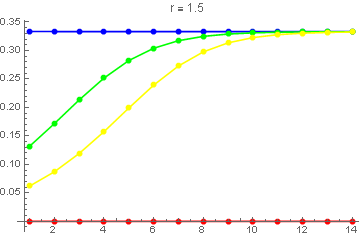
\includegraphics[clip=true,width=0.7\columnwidth]{a.r_1.5.png}
    \caption{Trayectorias para $r = 1.5$ y distintas condiciones iniciales $x_0$. Atractor: $x^* = 0.3335$.}
     \label{fig:a.r_1.5}
\end{figure}

A continuación se evaluó la trayectoria para $r = 2.9$. Como se observa en la figura \ref{fig:a.r_2.9}, la evolución es independiente de la condición inicial $x_0 \in (0,1]$. Además, el sistema tiene dos puntos fijos estables: $x^*=0$ y $0.6555$, siendo tan solo el segundo un atractor. A diferencia del caso anterior, la evolución hacia el atractor es oscilatoria y amortiguada.

\begin{figure}[htp]
    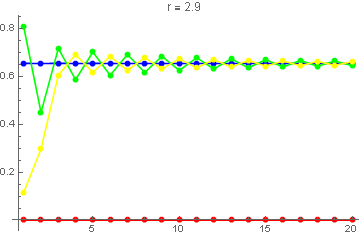
\includegraphics[clip=true,width=0.7\columnwidth]{a.r_2.9.png}
    \caption{Trayectorias para $r = 2.9$ y distintas condiciones iniciales $x_0$. Atractor: $x^* = 0.6555$.}
     \label{fig:a.r_2.9}
\end{figure}

Posteriormente, aumentando a $r = 3.3$, se encontró que la dinámica cambia completamente. Como se verifica en la figura \ref{fig:a.r_3.3}, no existe un único punto fijo sino dos que se repiten periódicamente: $x_1^* = 0.4795$ y $x_2^* = 0.8235$. Este cambio en la dinámica se denomina bifurcación de duplicación del período y la trayectoria se denomina período-2 o p-2. Este comportamiento se repite para valores de $r$ superiores. Este es el caso de $r = 3.5$ con trayectoria p-4 graficada en la figura \ref{fig:a.r_3.5} y de $r = 3.55$ con trayectoria p-8, en la figura \ref{fig:a.r_3.55}.

\begin{figure}[htp]
    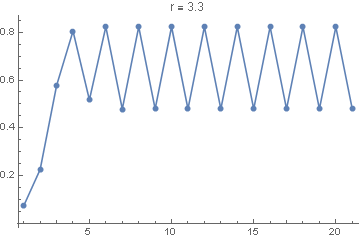
\includegraphics[clip=true,width=0.7\columnwidth]{a.r_3.3.png}
    \caption{Trayectoria $x_t$ para $r = 3.3$. El estacionario es idéntico para condiciones iniciales en el intervalo $(0,1]$. Dos atractores: $x^* = 0.8235$, $0.4795$.}
     \label{fig:a.r_3.3}
\end{figure}

\begin{figure}[htp]
    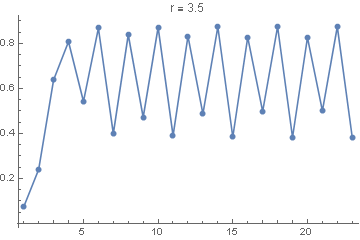
\includegraphics[clip=true,width=0.7\columnwidth]{a.r_3.5.png}
    \caption{Trayectoria para $r = 3.5$. El estacionario es idéntico para condiciones iniciales en el intervalo $(0,1]$. Cuatro atractores: $x^* = 0.3825$, $0.5005$, $0.8265$, $0.8745$.}
     \label{fig:a.r_3.5}
\end{figure}


\begin{figure}[htp]
    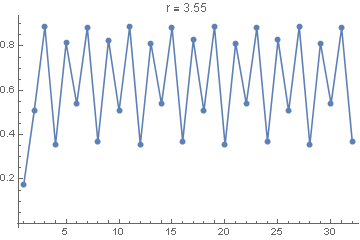
\includegraphics[clip=true,width=0.7\columnwidth]{a.r_3.55.png}
    \caption{Trayectoria para $r = 3.55$. El estacionario es idéntico para condiciones iniciales en el intervalo $(0,1]$. Ocho atractores: $x^* = 0.3545$, $0.3705$,  $0.5065$, $0.5405$, $0.8125$,  $0.8275$, $0.8815$, $0.8875$.}
     \label{fig:a.r_3.55}
\end{figure}

Para valores superiores del parámetro de control se presentan infinitos atractores como se observa en la figura \ref{fig:a.r_3.59} para $r = 3.59$. En este caso, los atractores son un continuo de puntos agrupados en dos intervalos y reciben el nombre de atractores caóticos. En la sección \ref{sec:d} se entrará en más detalle sobre qué se entiende por este último término.

\begin{figure}[htp]
    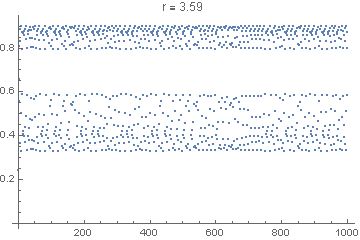
\includegraphics[clip=true,width=0.7\columnwidth]{a.r_3.59.png}
    \caption{Trayectoria $x_t$ para $r = 3.59$. No se conectaron los puntos de la trayectoria para facilitar la visualización.}
     \label{fig:a.r_3.59}
\end{figure}

Otro modo de visualizar los datos de la figura \ref{fig:a.r_3.59} es a través de un histograma de $x_t$ hasta un valor de $t_{max}$ predeterminado (ver figura  \ref{fig:a.histograma_3.59}). De este modo se logra visualizar fácilmente los valores visitados con mayor frecuencia durante la evolución del sistema y, además, permite visualizar desde otro punto de vista la dinámica caótica.

\begin{figure}[htp]
    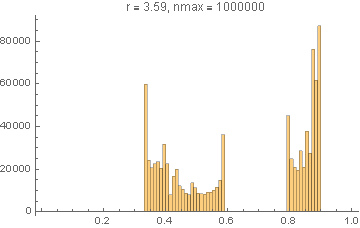
\includegraphics[clip=true,width=0.7\columnwidth]{a.histograma_3.59.png}
    \caption{Histograma de $x_t$ para $r = 3.59$.}
     \label{fig:a.histograma_3.59}
\end{figure}


El mismo procedimiento para $r$ mayores indica un comportamiento similar. Sin embargo, para determinados valores ocurren comportamientos regulares. Este es el caso de $r = 3.83$ con una tractoria p-3 graficada en la figura \ref{fig:a.r_3.83}. Esta presenta tan solo tres atractores como se verifica en el histograma de la figura \ref{fig:a.histograma_3.83}. Aumentando ligeramente $r$ se vuelve al comportamiento caótico. $r$ no puede aumentar indefinidamente. El límite está dado por $r = 4.$ en el que todos los puntos del intervalo $(0,1]$ son atractores pero son visitados con distinta frecuencia (trayectoria en la figura \ref{fig:a.r_4} e histograma en la \ref{fig:a.histograma_4}). Para valores superiores la solución diverge.

\begin{figure}[htp]
    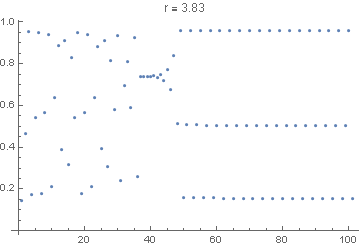
\includegraphics[clip=true,width=0.7\columnwidth]{a.r_3.83.png}
    \caption{Trayectoria $x_t$ para $r = 3.83$. No se conectaron los puntos de la trayectoria para facilitar la visualización.}
     \label{fig:a.r_3.83}
\end{figure}

\begin{figure}[htp]
    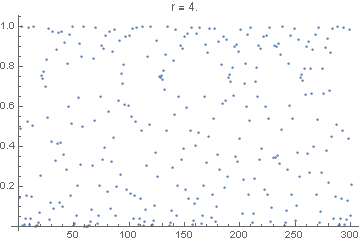
\includegraphics[clip=true,width=0.7\columnwidth]{a.r_4.png}
    \caption{Trayectoria $x_t$ para $r = 4$. No se conectaron los puntos de la trayectoria para facilitar la visualización.}
     \label{fig:a.r_4}
\end{figure}

\begin{figure}[htp]
    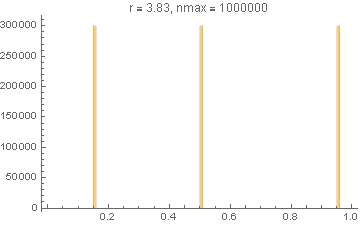
\includegraphics[clip=true,width=0.7\columnwidth]{a.histograma_3.83.png}
    \caption{Histograma de $x_t$ para $r = 3.83$.}
     \label{fig:a.histograma_3.83}
\end{figure}

\begin{figure}[htp]
    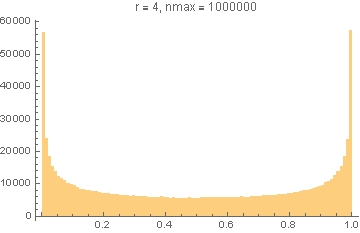
\includegraphics[clip=true,width=0.7\columnwidth]{a.histograma_4.png}
    \caption{Histograma de $x_t$ para $r = 4$.}
     \label{fig:a.histograma_4}
\end{figure}


\section{\label{sec:b}Diagrama cobweb}

Otro modo de representar la evolución del sistema es el diagrama cobweb. En este se grafica la función
\[f(x) = r x (1-x),\]
la identidad y una órbita que representa la trayectoria del sistema. Por ejemplo,  para $r = 2.22$ se botuvo el gráfico de la figura \ref{fig:b.cobweb.r_2.22}. En este se observa claramente el atractor estable $x^* = 0.5495$. Algebraicamente, el criterio para determinar la estabilidad de un punto fijo $x^*$ en un mapeo $f$ es el siguiente:
\begin{itemize}
    \item Si $\mid f^{\prime} (x^{*})\mid < 1$ el punto es estable.
    \item Si $\mid f^\prime(x^*)\mid > 1 $ el punto es inestable.
    \item Si  $\mid f^\prime(x^*)\mid = 1 $ el criterio no aporta información.
\end{itemize}
En este caso, $f^\prime(x) = r(1 - 2x)$ y los puntos fijos $x^*$ son aquellos en los que se cumple $x_t = r x_t (1-x_t)$, en otras palabras $f(x^*) = x^*$.

\begin{figure}[htp]
    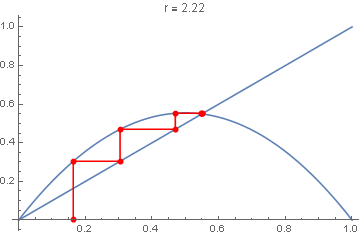
\includegraphics[clip=true,width=0.7\columnwidth]{b.cobweb.r_2.22.png}
    \caption{Diagrama cobweb para $r = 2.22$.}
     \label{fig:b.cobweb.r_2.22}
\end{figure}

Hay dos puntos que cumplen esta condición: $x^* = 0$, $(r-1)/r$. El criterio de estabilidad aplicado al primero de ellos indica $f'(0) = r$. Entonces, este punto será estable para $r<1$ e inestable para valores mayores. Mientras que para el segundo, $f'( (r-1)/r ) = 2 - r$ y se concluye que este punto será inestable para $r<1$ pero estable para $1<r<3$. Este comportamiento fue el encontrado al analizar las figuras \ref{fig:a.r_1.5} y \ref{fig:a.r_2.9}. Cabe preguntarse qué ocurrirá para $r$ mayores. La figura \ref{fig:a.r_3.3} indica una trayectoria p-2, la cual también se ve reflejada en el diagrama cobweb de la figura \ref{fig:b.cobweb.r_3.3}. En este se observa que la trayectoria p-2 cumple en el estado estacionario una nueva condición: $f(x_1^*) = x_2^*$, $f(x_2^*) = x_1^*$, es decir, $f(f(x_1^*)) = x_1^*$. La trayectoria es un punto fijo del mapeo $x_{n+1} = f(f(x_n)) = f^2(x_n)$. Consecuentemente, para analizar la estabilidad se deberá aplicar el criterio a $f^2$. En primer lugar, hay cuatro valores que cumplen $f^2(x) = x$ dado que es polinomio de grado cuatro. Dos de sus raíces son inestables para $r<3$ y las otras dos, dadas por la expresión
\[x_{1,2}^* = \frac{ 0.5(r + r^2 \pm r \sqrt{-3 -2 r + r^2})}{r^2},\]
son estables para $3 < r < 3.4495 $: $f^{2 \prime} (x_1^{*}) = f^{2 \prime} (x_2^{*}) = -r^2 + 2 r + 4$. Para $r$ mayores ocurre el mismo fenómeno: los puntos fijos se vuelven inestables y el diagrama cobweb (figura \ref{fig:b.cobweb.r_3.5}) indica que la trayectoria p-4 cumple en el estado estacionario la condición $f^{2}(f^2(x)) = f^4(x) = x$. Para $r$ mayores se tiene la trayectoria p-8 (ver figura \ref{fig:b.cobweb.r_3.55}) y sucesivamente.Se puede ver que a modo general la trayectoria p-n es un punto fijo estable de la iteración $f^{2n}$.

\begin{figure}[htp]
    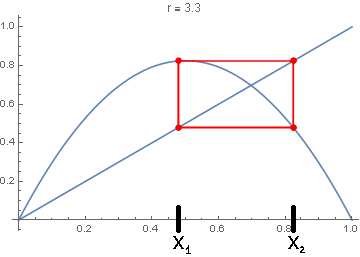
\includegraphics[clip=true,width=0.7\columnwidth]{b.cobweb.r_3.3.png}
    \caption{Diagrama cobweb para $r = 3.3$. El transitorio no fue graficado para una mejor visualización.}
     \label{fig:b.cobweb.r_3.3}
\end{figure}

\begin{figure}[htp]
    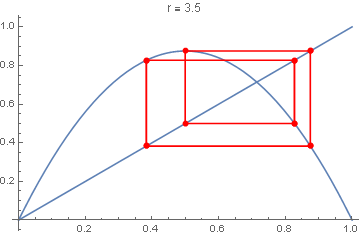
\includegraphics[clip=true,width=0.7\columnwidth]{b.cobweb.r_3.5.png}
    \caption{Diagrama cobweb para $r=3.5$. El transitorio no fue graficado para una mejor visualización.}
     \label{fig:b.cobweb.r_3.5}
\end{figure}

\begin{figure}[htp]
    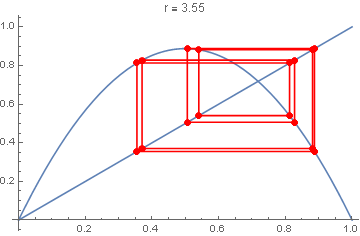
\includegraphics[clip=true,width=0.7\columnwidth]{b.cobweb.r_3.55.png}
    \caption{Diagrama cobweb para $r=3.55$. El transitorio no fue graficado para una mejor visualización.}
     \label{fig:b.cobweb.r_3.55}
\end{figure}

\begin{comment}

\begin{figure}[h]
    \includegraphics[clip=true,width=\columnwidth]{.png}
    \caption{.}
     \label{fig:}
\end{figure}

Inciso b
Descripción de esta nueva representación

Descripción de la inestabilidad

Descripción de la primera inestabilidad hacia p-2

Descripción de la segunda inestabilidad hacia p-4

Descripción de la segunda inestabilidad hacia p-8




\end{comment}


\section{\label{sec:c}Diagrama de bifurcaciones}

En secciones anteriores se identificaron los atractores para determinados valores de $r$. Sistemáticamente se realizó esta identificación para distintos valores del parámetro en el intervalo $[1,4]$. Los resultados obtenidos se graficaron en la figura \ref{fig:c_diag_bif_r_1}. Existen varios fenómenos discutidos anteriormente que se reflejan en este diagrama y aparecen además algunos nuevos. En primer lugar, se observa claramenta el fenómeno de bifurcación de período. Por ejemplo, en $r = 3.3$ aproximadamente cuando partiendo de un único atractor, la dinámica cambia, el camino se bifurca y aparece otro atractor. En segundo lugar, los valores $r_i$ donde se dan dichas bifurcaciones de período se acumulan sucesivamente hasta $r_\infty$ donde los atractores se convierten en un continuo. Para valores superiores la dinámica se vuelve caótica con algunas ventanas de comportamiento regular como es el caso de $r = 3.83$. En tercer lugar, cerca de los puntos de bifurcación es complicado identificar los atractores dado que estos cambian rápidamente para valores próximos de $r$ y, además, los transitorios correspondientes son más largos. En cuarto lugar, se observa la presencia estructuras autosemejantes, es decir, el diagrama se repite a distintas escalas. Esto se observa claramente en la figura \ref{fig:c_diag_bif_rs} donde el primer gráfico corresponde al intervalo $r \in (3$,$3.678)$, el segundo a $r \in (3.45122$, $3.59383)$ y el tercero, $r \in  (3.54416$, $3.57490)$.

\begin{figure}[htp]
    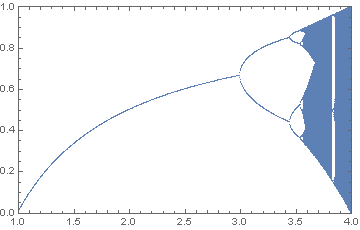
\includegraphics[clip=true,width=0.7\columnwidth]{c_diag_bif_r_1.png}
    \caption{Diagrama de bifurcaciones.}
     \label{fig:c_diag_bif_r_1}
\end{figure}

\begin{figure}[htp]
    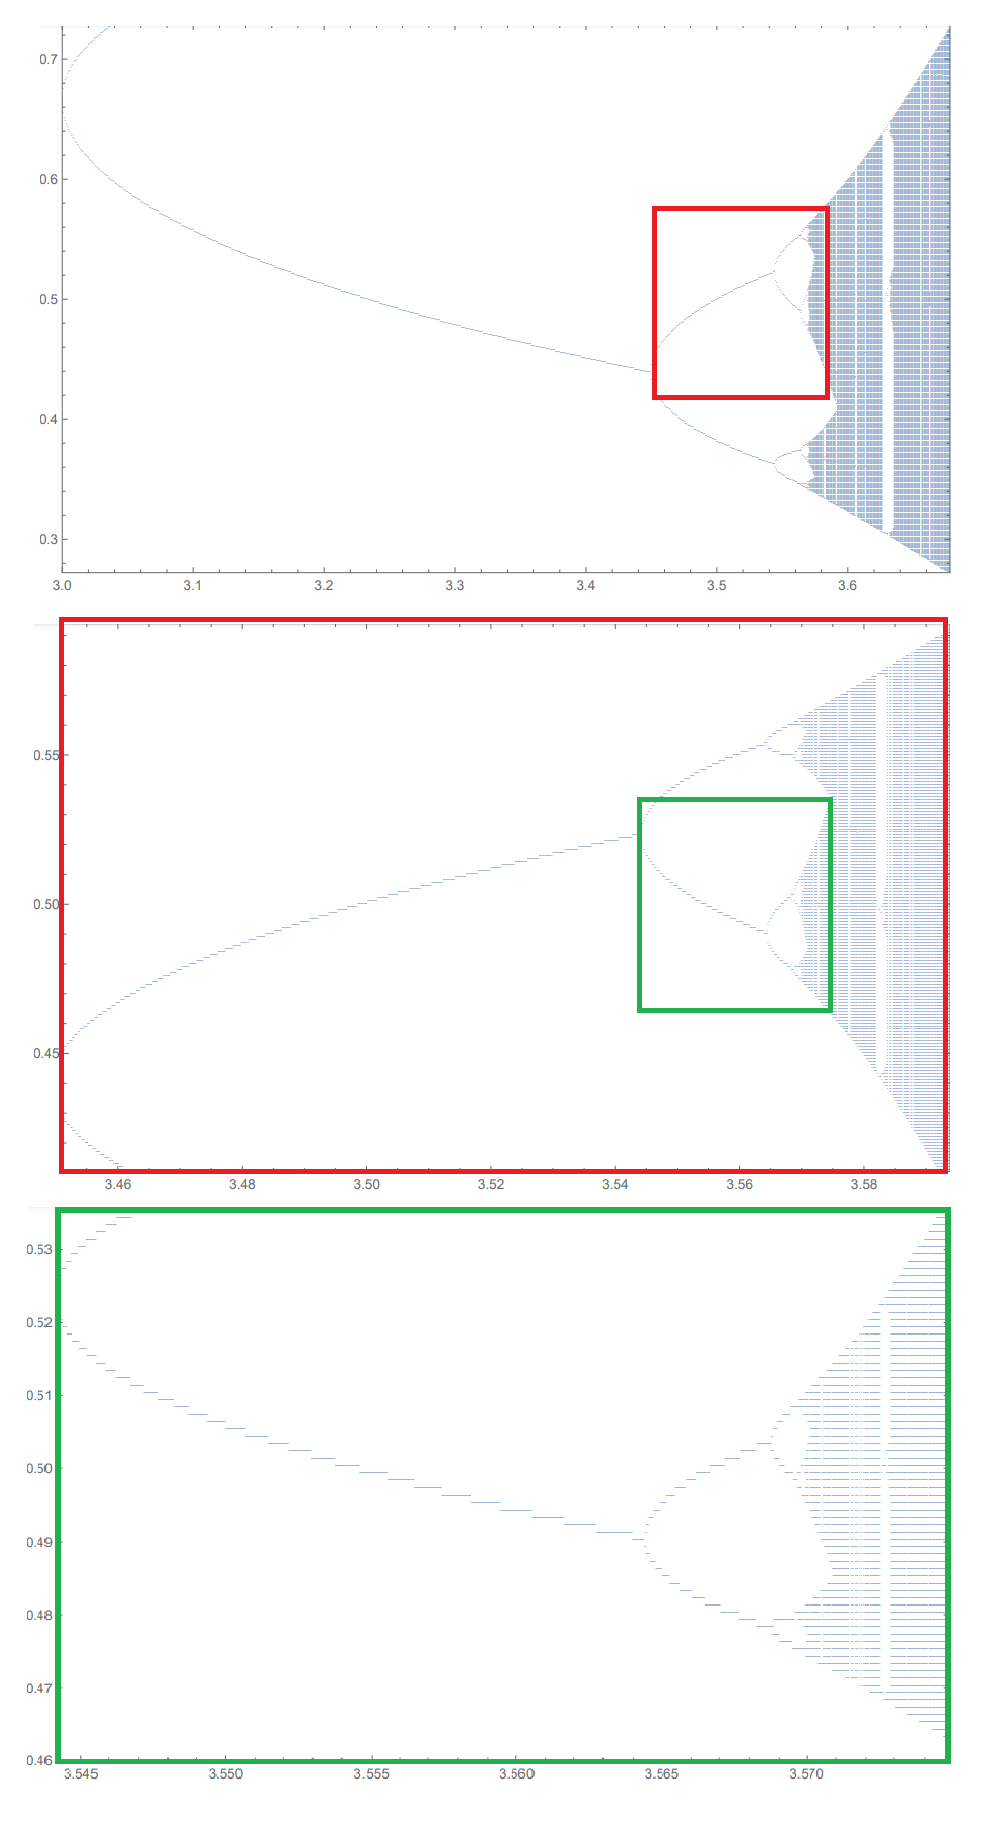
\includegraphics[clip=true,width=0.6\columnwidth]{c_diag_bif_rs.png}
    \caption{Diagrama de bifurcaciones para distintas escalas.}
     \label{fig:c_diag_bif_rs}
\end{figure}

\section{\label{sec:d}Exponenente de Lyapunov}

Como se mencionó anteriormente, para $r > r_\infty \approx 3.568$ el sistema es caótico. Esto se caracteriza por la sensibilidad a las condiciones iniciales, es decir, condiciones iniciales cercanas generan trayectorias que se separan rápidamente. Esta separación se puede caracterizar a través del exponente de Lyapunov $\lambda$ dado por
\[ |\Delta x_t | = |\Delta x_0 | e^{\lambda t},\]
donde $\Delta x_t$ representa la diferencia entre los valores de $x_t$ correspondientes a condiciones iniciales distanciadas en $\Delta x_0$. De este modo, si $\lambda > 0$ las trayectorias se separan y la dinámica es caótica. Mientras que si $\lambda < 0$, se está en presencia de comportamiento regular: trayectorias cercanas son cada vez más cercanas. Por último, si $\lambda \approx 0$, $\Delta x_t$ varía lentamente y, consecuentemente, el transitorio es lento.

$\lambda$ se puede determinar explícitamente para distintos valores de $r$ a partir de la expresión
\[\lambda = \frac{1}{n} \sum_{i = 0}^{n-1}\ln{|f'(x_i)|}.\]
Los resultados se grafican en la figura \ref{fig:d.lambda}. En base al valor de $\lambda$ se pueden reproducir resultados que se obtivieron en secciones anteriores. En primer lugar, para $r < r_\infty$, $\lambda < 0$ y el comportamiento es regular salvo para algunos puntos donde $\lambda = 0$. Estos últimos corresponden a los puntos de bifurcación de duplicación de período y se caracterizan por un largo transitorio. En segundo lugar, para $r > r_\infty$, $\lambda > 0$ y el comportamiento es caótico salvo para ciertas regiones de comportamiento regular donde ocurre lo contrario.

\begin{figure}[htp]
    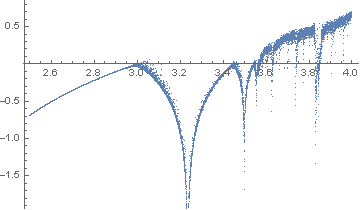
\includegraphics[clip=true,width=0.7\columnwidth]{d.lambda.png}
    \caption{Exponenente de Lyapunov $\lambda$ en función de $r$.}
     \label{fig:d.lambda}
\end{figure}


Ventanas de comportamiento regural


\bibliography{Radiacion_de_cuerpo_negro}

\end{document}

